\documentclass{article}

\usepackage[utf8]{inputenc}
\usepackage{graphicx}
\usepackage{caption}
\usepackage{listings}
\usepackage{lastpage}

\usepackage{hyperref}
\urlstyle{same}

\usepackage[export]{adjustbox} %center

% pakiety do języka polskiego
\usepackage[T1]{fontenc}
\usepackage[polish]{babel}
\usepackage[utf8]{inputenc}

\usepackage{indentfirst} % wcięcia

\captionsetup[figure]{name={caption}}

\title {Specyfikacja Implementacyjna Projektu ,,Optymalizacja Dostaw Szczepionek'' VAM} 
\author{Bartosz Zakrzewski}
\date{Data utworzenia 18.11.2020 \\ Data ostatniej modyfikacji 19.11.2020}

% Nagłówki na każdej stronie:
\usepackage{fancyhdr}
\pagestyle{fancy}
\fancyhf{}
\rhead{Bartosz Zakrzewski}
\lhead{Specyfikacja Impl. ,,Optymalizacja Dostaw Szczepionek''}
\rfoot{Strona \thepage \hspace{1pt} z \pageref{LastPage}}

\begin{document}
\maketitle
\thispagestyle{empty}

\clearpage
\tableofcontents
\thispagestyle{empty}

\clearpage

\section{Cel Projektu}
Celem projektu jest napisanie programu, który sprawi, że apteki kupią takie ilości szczepionek, od różnych producentów, za poszczególne ceny tak, że łączny koszt za wszystkie szczepionki będzie najmniejszy.

\section{Uruchomienie programu}

Aby program mógł wykonać obliczenia, należy dostarczyć do niego plik wejściowy poprawnie sformatowany i zawierający poprawne wartości.
\\

\par Jeżeli błąd wystąpi, program wypisze pierwszy napotkany błąd na konsolę i do pliku o nazwie ,,error.txt''. W przeciwnym razie użytkownik otrzyma plik wyjściowy o nazwie ,,optymalizacja.txt''.
Aby użytkownik mógł odnaleźć błąd w pliku wejściowym, program poinformuje, w jakiej linii znalazł go i jakiego rodzaju to był błąd.
\\ 
\par Uruchomienie następuje za pomocą java -jar:

\begin{lstlisting}
java -jar Optymalizacja.jar nazwa_pliku_wejsciowego.txt
\end{lstlisting}

\section{Środowisko pracy}
Program będzie implementowany na jednym komputerze przez jedną osobę.

\begin{itemize}
    \item System operacyjny - Windows 10
    \item IDE - Intellij IDEA 2020.2.3 Community Edition
    \item Java 14 (JDK 14)
    \item JUnit 4.13
    \item System kontroli wersji git, repozytorium umieszczone na platformie ISOD
\end{itemize}

\clearpage

\section{Zasady wersjonowania i językowe}
\begin{itemize}
    \item Commity będą po angielsku.
    \item Kod będzie pisany w języku angielskim.
    \item Gałęzie będą miały nazwę zaczynającą się od numeru porządkującego i słowa będą oddzielone znakiem ,,\_'' np. 04\_Find\_minimal\_difference.
    \item Odstępstwa od języka angielskiego mogą występować, gdy znaczenie w języku polskim jest unikalne: np. nazwy specyfikacji: gałąź o nazwie 01\_Specyfikacja\_Funkcjonalna.
    \item Jeżeli posługiwanie się językiem polskim ułatwi implementację, to można go użyć, np. używanie nazwy Apteka zamiast Pharmacy.
    \item Commity mogą zostać otagowane, jeżeli zajdzie taka potrzeba.
\end{itemize}

\section{Wygląd pliku wejściowego i wyjściowego}

\begin{figure} [hbt!]
    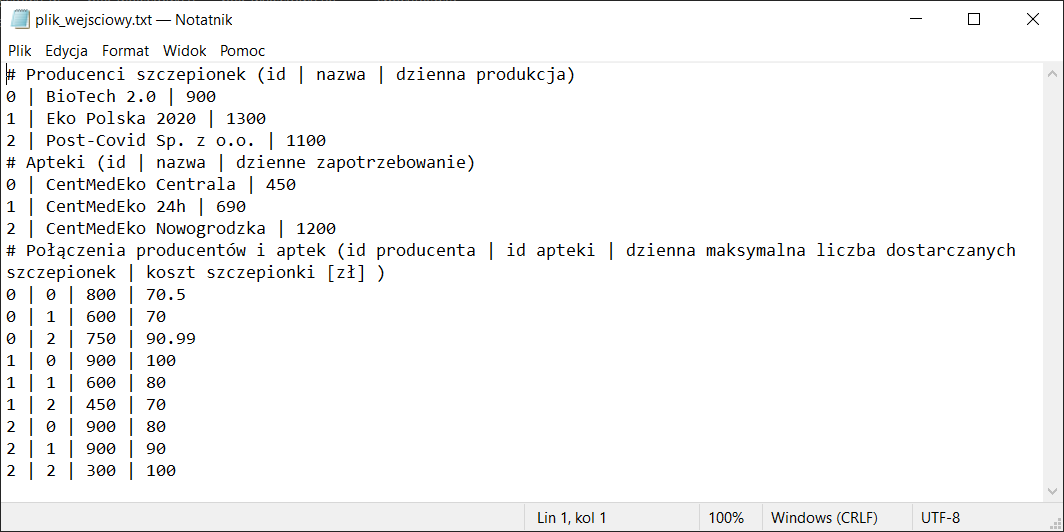
\includegraphics[width=15cm,center]{images/plik_wejsciowy.PNG}
    \captionof{figure}{Przykładowy plik wejściowy}
\end{figure}

\begin{figure} [hbt!]
    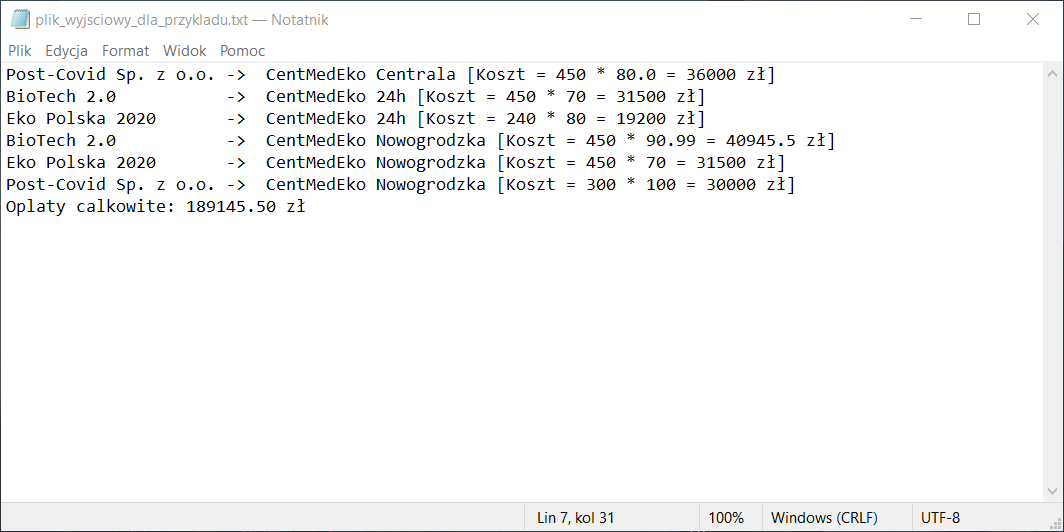
\includegraphics[width=15cm,center]{images/plik_wyjsciowy_dla_przykladu.PNG}
    \captionof{figure}{Przykładowy plik wyjściowy}
\end{figure}

\section{Analiza algorytmu}
Implementacja programu własnym sposobem została przerwana na rzecz implementacji metody VAM (Vogel’s Approximation Method) (Zagadnienie transportowe).

\begin{figure} [hbt!]
    \includegraphics[width=15cm,center]{images/implementacja została przerwana.PNG}
    \captionof{figure}{Implementacja programu własnym sposobem została przerwana}
\end{figure}

\url{https://www.youtube.com/watch?v=WQdW9jLiPZg&ab_channel=PlusProjekt}
\url{http://kmp.wm.tu.koszalin.pl/cms/dydaktyka/atomkowska/atomkowska_22.pdf}

\clearpage

\section{Źródła}

\begin{itemize}
    \item Opis problemu, przykładowy plik wejściowy i wyjściowy przygotował i umieścił na platformie ISOD mgr inż. Paweł Zawadzki
    \item Rysunki poglądowe zostały wykonane za pomocą programu Paint 3D
    \item Ten dokument został stworzony na stronie overleaf.com
    \item \url{https://www.youtube.com/watch?v=WQdW9jLiPZg&ab_channel=PlusProjekt}
    \item \url{http://kmp.wm.tu.koszalin.pl/cms/dydaktyka/atomkowska/atomkowska_22.pdf}
\end{itemize}

\end{document}